\chapter{Extending our work to Deep CCA and Self-Supervised Learning: A Powerful Approach to Multiview Nonlinear Association Learning}
\label{Deep}

\section{Introduction}


\section{Background and Related Work}

\subsection{Deep Learning}

With large amounts of data and improvements in hardware in recent years, `Deep' neural networks have become the state of the art in many tasks and in particular in computer vision. In principle, an infinitely wide neural network could model any function to arbitrary accuracy - a property known as the universal approximation theorem - and this flexibility allows neural networks to model complex relationships. 

In practice, rather than infinitely wide networks, `Deep' Neural Networks combine layers of linear weights with non-linear activation functions. Each layer can generally be written as a function of the outputs of the previous layer (or the raw input for the first layer):

$$
\bold{h_i}=s_i(\bold{W_ih_{i-1}}+\bold{b_i})
$$

Where we use the letter $h$ to denote a `hidden' layer or a representation between the input and output, $W$ to represent a matrix of weights, $b_i$ to represent a vector of bias terms and $s$, critically, to represent a non-linear activation function. One example of a non-linear activation function is the sigmoid function which maps linear outputs to a value between 0 and 1. Neural networks are often designed to have bottlenecks with fewer features in each subsequent hidden layer. This means that the outputs of each layer produce a hierarchy of features and it is often hypothesized that their generalisation ability is built upon producing these layers of abstraction\cite{li2018survey}. In general we will refer to the complete set of parameters (and architectural choices such as the number of layers) in a neural network with $\theta$. We therefore write a neural network function as $F(\bold{X};\theta_F)$.

The most common way to optimize neural networks is to use gradient descent (GD) in which we calculate the gradient of the network parameters with respect to some objective. When using the whole dataset to calculate the gradient we typically refer to `batch' gradient descent. However, when using non-linear functions, the objective is typically non-convex meaning GD is prone to finding local minima (regions in the parameter space where the gradient of the objective is zero) rather than global minima (local minima where the value of the objective is optimal). Perhaps for this reason, it is more effective to use Stochastic Gradient Descent (SGD), in which we estimate the gradient by using a single sample or a small set of samples referred to as a `minibatch'. This noisy estimate is less likely to get `stuck' in suboptimal solutions. Stochastic gradient descent mathematically relies on the stochastic estimate of the gradient being an unbiased estimate of the true gradient.

\subsection{Deep CCA}

Deep Canonical Correlation Analysis provides an alternative method to kernel CCA for finding complex non-linear structure in multiview data \cite{andrew2013deep}. In Deep CCA we look to use functions parameterized by neural networks $F(\bold{X};\theta_F)$ and $G(\bold{Y};\theta_G)$ to map the original data into a space in which the two views are maximally correlated. The problem we would like to solve is therefore:

\begin{align}
    & \theta_{F_{opt}},\theta_{G_{opt}}=\mathrm{argmax}\{\text{trace}( F(\bold{X};\theta_F)^{\top}G(\bold{Y};\theta_G))  \}\\
    & \text{subject to:} \notag\\
    & F(\bold{X};\theta_F)^{\top}F(\bold{X};\theta_F)=1 \notag\\
    & G(\bold{Y};\theta_G)^{\top}G(\bold{Y};\theta_G)=1 \notag
\end{align}

As we showed earlier in section \ref{sec:cca}, sum of the top $k$ canonical correlations of two views of a dataset can be shown to be the sum of the top $k$ singular values of the matrix $\bold{T}=\bold{\Sigma_{11}^{-\frac{1}{2}}\Sigma_{12}\Sigma_{22}^{-\frac{1}{2}}}$ where $\Sigma_{11}=F(\bold{X};\theta_F)^{\top}F(\bold{X};\theta_F)$. Now consider the identity $\|\bold{T}\|_*=\text{tr}(\sqrt{\bold{T^{\top}T}})$ known as the tracenorm of $\bold{T}$. This is symmetric and therefore can be diagonalised. Then since $T=\bold{U\Sigma V^{\top}}$:

\begin{align}
    & \|\bold{T}\|_*=tr(\sqrt{\bold{V\Sigma U^{\top}U\Sigma V^{\top}}})=tr(\sqrt{\bold{\Sigma^2 VV^{\top}}})=tr(\bold{\Sigma})
\end{align}

Therefore maximising the tracenorm maximises the total correlation between the representations.

\begin{figure}[H] %[H] "corresponds to start the figure Here"
    \centering %alignment can be flushleft, centering or flushright
    %includegraphics is the command to include graphics or pictures, [Width should be defined with respect to textwidth]{The path/ location of the image in the specified folder}, the image should be either in .png, .jpg, .pdf formats faster processing
    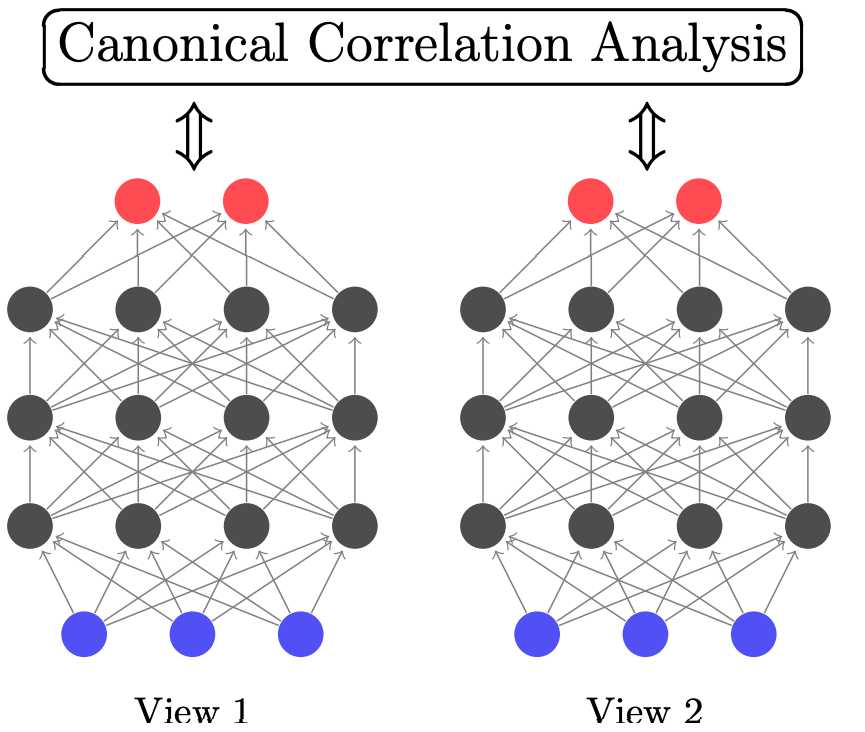
\includegraphics[width=0.5\textwidth]{chapters/litreview/DCCA.png} 
    \caption[Deep CCA Representation]{\textit{\textbf{Deep CCA with two correlated dimensions:}} A separate neural network is learnt for each view and a linear CCA is applied on top \cite{andrew2013deep}}
    \label{img:DCCA}
\end{figure}

A major problem with this DCCA formulation is that it relies on full-batch optimisation (optimized in the original paper by using the L-BFGS optimization algorithm). When gradients are calculated using smaller minibatches, the performance degrades drastically  because the estimation of the gradient is biased. In particular, mathematically the terms in $\Sigma_{ii}^{-\frac{1}{2}}$ are overestimated due to Jensen's inequality $E[\frac{1}{X}]>\frac{1}{E[X]}$. More intuitively, these matrices may be near singular for small samples causing stochastic gradients to blow up.

\subsection{Self-Supervised Learning}
\subsubsection{Barlow Twins}
%Relationship to CCA

\subsubsection{VICReg}
%Likewise


It is well known that VICReg and Barlow twins are closely related to CCA \cite{balestriero2022contrastive}. Similarly, \cite{kiani2022joint} showed how the SSL losses like VICReg could be adapted and implemented in closed form using the kernel method. Our work approaches the problem from the opposite angle, demonstrating how these classical problems can be extended to deep learning and solved with SGD without introducing bias.

\section{Methods}

\subsection{DCCA-EY and DCCA-SVD: Extension to Deep CCA}\label{sec:deep-cca}
The GEP-EY and CCA-SVD formulations also lead naturally to new formulations of Deep CCA which solve a more flexible CCA problem but unlike prior work can be optimized efficiently in the stochastic setting. We will refer to these as DCCA-EY and DCCA-SVD.

%L; just moved this up
We derive the DCCA-EY formulation by applying the GEP formulation of CCA (\ref{eq:cca-GEV}) to our DCCA definition. The analogous derivation for DCCA-SVD is left to supplement \ref{supp:algorithm-details}. 

Population DCCA \cite{andrew2013deep} can be defined analogously to population CCA (see section \ref{sec:CCA Definition}):
% Following the definition of CCA in section \ref{sec:CCA Definition}, the population formulation of DCCA \cite{andrew2013deep}, can be defined as follows: 
given input random vectors $X \in \R^{D_x}, Y \in \R^{D_y}$, find neural networks $f,g$ maximising:
\begin{align}\label{eq:DCCA-Andrew}
    \max_{f,g}  \norm{\CCA_K\left(f(X),g(Y)\right)}_2
\end{align}
% \in \mathcal{F}, g \in \mathcal{G}
% First we need to define the relevant matrices for our GEP. Consider $f,g$ as fixed for now, and define the (population) covariance matrices $\Sigma_{ff} = \operatorname{Var}(f(X)),\Sigma_{f,g} = \operatorname{Cov}(f(X),g(Y)),\Sigma_{gg}=\operatorname{Var}(g(Y))$. Then take
% \begin{equation*}
%     A_{fg} = \begin{pmatrix} 0 &\Sigma_{fg} \\ \Sigma_{gf} & 0 \end{pmatrix}, \qquad
% 	B_{fg} = \begin{pmatrix}\Sigma_{ff} & 0 \\ 0 & \Sigma_{gg}\end{pmatrix}
% \end{equation*}

The GEP formulation becomes:
\begin{equation*}
    A_{fg} = \begin{pmatrix} 0 &\Cov(f(X),g(Y)) \\ \Cov(g(Y),f(X)) & 0 \end{pmatrix}, \qquad
	B_{fg} = \begin{pmatrix}\Var(f(X)) & 0 \\ 0 & \Var(g(Y)) \end{pmatrix}.
\end{equation*}

Proposition \ref{prop:EY-charac} then allows us to rewrite our objective (\ref{eq:DCCA-Andrew}) as:
\begin{align*}
    % not quite equivalent to Andrew version without 1 extra small result
    %\max_{f \in \mathcal{F}, g \in \mathcal{G}}  \norm{\CCA_K\left(f(X),g(Y)\right)}_2
    %\max_{f,g,W} 
    \norm{\CCA_k\left(f(X),g(Y)\right)}^2 
    = \sum_{j=1}^k \rho_j^2 
    = \max_{W \in \R^{d \times k}} \tr \left( 2\, W^T A_{fg} W - \left(W^T B_{fg} W\right) \left(W^T B_{fg} W\right) \right).
\end{align*}
Therefore DCCA is equivalent to maximising the right hand side with respect to $f,g$ and $W$. To simplify the objective we follow \cite{wang2015stochastic} and reparametrize to consider the `augmented' neural networks $\bar{f} = U^{\top} f, \bar{g} = V^{\top} g$, where $U\in \R^{d_x \times k}, V\in \R^{d_y \times k}$ are such that $W^{\top} = (U^{\top}, V^{\top})$. This gives our final DCCA objective:

\begin{align}\label{eq:DCCA-EY}
    \mathcal{U}^\text{DCCA-EY}(\bar{f},\bar{g}) = \tr(2 \, A_{\bar{f}\bar{g}} - B_{\bar{f}\bar{g}} B_{\bar{f}\bar{g}})
\end{align}

where we need to define:
\begin{align*}
    A_{\bar{f}\bar{g}}
    &= W^T A_{fg} W 
    = \Cov(\bar{f}(X),\bar{g}(Y)) + \Cov(\bar{g}(Y),\bar{f}(X)) \\
    B_{\bar{f}\bar{g}} 
    &= W^T B_{fg} W 
    = \Cov(\bar{f}(X)) + \Cov(\bar{g}(Y))
\end{align*}

%L: there is a key difference in focus here - no longer have that the gradients are super cheap to compute in terms of the matrix dimensions, the dominant cost is going to be backprop through potentially fat $f,g$ rather than the final layer of $W$.
By plugging in sample covariances on a minibatch, we can obtain unbiased estimates of $\mathcal{U}^\text{DCCA-EY}(\bar{f},\bar{g})$.
% L: this is nit-picking and maybe obvious, but I missed it first time.
Therefore, we can apply some variant of SGD to optimize equation \ref{eq:DCCA-EY}.

Note that, as in the earlier DCCA work, though we derived the algorithm by considering $f,g$ with output dimensions $d_x,d_y$, we ultimately end up with networks $\bar{f},\bar{g}$ with the same output dimension $k$; we can view these as giving highly correlated $k$-dimensional embeddings of our data.
% Old: Note that, as in the earlier DCCA work, we ultimately end up with networks $\bar{f},\bar{g}$ which give us $k$ dimensional `latent' representations of our data. 
% L: I wrote this before but am no longer sure what it is doing here. There's something subtle about starting with $d_x$ NN outputs and only keeping $k$ directions...but it's what was done before

%maybe need extra stress on the interchange of expectation and differentiation / why it works, but maybe that's fine

%%% Unused ackground copied and pasted from Generalized Eigengame paper
%%% potentially will want to add in: 

% %augmented objective classes
% \begin{equation*}
%     \tilde{\mathcal{F}} = \{\bar{f} = U^{\top} f : f \in \mathcal{F}, U\in \R^{d_x \times k}\}, \quad
%     \tilde{\mathcal{G}} = \{\bar{g} = V^{\top} g : g \in \mathcal{G}, V\in \R^{d_y \times k}\}
% \end{equation*}

% % why putting tilde's on the Sigma's makes sense
% \begin{equation*}
%     U^{\top} \Sigma_{ff} U = \Sigma_{\bar{f}\bar{f}}, \quad
%     U^{\top} \Sigma_{fg} U = \Sigma_{\bar{f}\bar{g}}, \quad
%     V^{\top} \Sigma_{gg} V = \Sigma_{\bar{g}\bar{g}}
% \end{equation*}

\subsection{SSL-EY and SSL-SVD: Application to Self-Supervised Learning}

Finding highly correlated embeddings is a natural objective for SSL.
To apply the previous ideas to joint embedding methods, we simply apply (\ref{eq:DCCA-EY}) in the Siamese pair setting where $\bar{f}=\bar{g}$ are the same map from input data to embeddings (composition of encoder and projector).

% To apply these ideas to SSL, we suppose that our latent representations are learnt by 
% Finally, we introduce SSL-EY and SSL-SVD which adapt DCCA to the SSL setting in a principled way which permits greater understanding and, as we shall see, informs architecture choice.

% Following the 

% \begin{align*}
%     \tr 2 \left( \Cov(Z,Z') + \Cov(Z',Z) \right) - ...
% \end{align*}
% Consider the $f = h \circ g$ the encoder-expander composition.
% We will then apply (\ref{eq:DCCA-EY}) in the Siamese pair setting standard in SSL to enforce our embeddings to be highly correlated.

%Previously $X,Y$ were fundamentally different objects and we wanted to learn their relationship. In the SSL setting, we have $X, X'$ which are augmentations of the same object and we want to learn an embedding that is invariant to our data augmentations. For this reason, as is standard in SSL for computer vision, both views $X,X'$ share a neural network $f$.

We therefore obtain the objective:
\begin{align}\label{eq:SSL-EY}
    \mathcal{U}^\text{SSL-EY}(\bar{f}) =\tr( 2 \, A_{\bar{f}} - B_{\bar{f}} B_{\bar{f}})
\end{align}
where:
\begin{align*}
    A_{\bar{f}}
    &= \Cov(\bar{f}(X),\bar{f}(X')) + \Cov(\bar{f}(X'),\bar{f}(X)) \\
    B_{\bar{f}} 
    &= \Var(\bar{f}(X)) + \Var(\bar{f}(X')).
\end{align*}

Once again, we define SSL-SVD by analogy in supplement \ref{supp:algorithm-details}. We will see in section \ref{Experiments} that SSL-SVD and SSL-EY perform similarly in experiments but we show in supplement \ref{supp:previous work} that the SSL-SVD formulation looks closer to existing SSL methods.

\textbf{Implementation Details:} Typical architectures for the encoder and the projector vary depending on the domain and the dataset \cite{balestriero2023cookbook}. For example, for image classification tasks on CIFAR-10 or ImageNet, a common choice for the encoder is a ResNet, while for the projector a linear layer or a two-layer MLP is often used. Common augmentations for images are cropping, flipping, rotating, color jittering, etc. In this work, we adopt standard architectures and augmentations from the literature.


\section{Experiments and Results}

%%%%%%%%%%%%%%%%%%%%%%%%%%%%%%%%%%%%%%%%%%%%%%%%%%%%%%%%%%%%%%%%%%%%%%%%%%%%%%%%%%%%%%
%DCCA Benchmarking
%%%%%%%%%%%%%%%%%%%%%%%%%%%%%%%%%%%%%%%%%%%%%%%%%%%%%%%%%%%%%%%%%%%%%%%%%%%%%%%%%%%%%%
\subsection{Application of DCCA-EY and DCCA-SVD to to Deep multiview learning on toy data}

We now turn to compare our proposed DCCA-EY and DCCA-SVD methods with existing methods for deep canonical correlation analysis (DCCA). We replicate an experiment from \cite{wang2015stochastic} using the left and right halves of MNIST \cite{lecun1998gradient} digits ($n$=60,000) and X-Ray Microbeam (XRMB, $n$=1,429,236) data \cite{westbury1994x}. XRMB is a multimodal dataset of speech recordings from 139 speakers with acoustic and articulatory features. We use minibatch sizes of 100 for 20 epochs, the architectures described in \cite{wang2015stochastic}, and an output dimensionality of 50.  We use the total correlation captured (TCC) of the learnt subspace on the validation set as a metric (defined in supplement \ref{supp:experimental details}).

\begin{figure}
     \centering
     \begin{subfigure}[b]{0.49\textwidth}
         \centering
         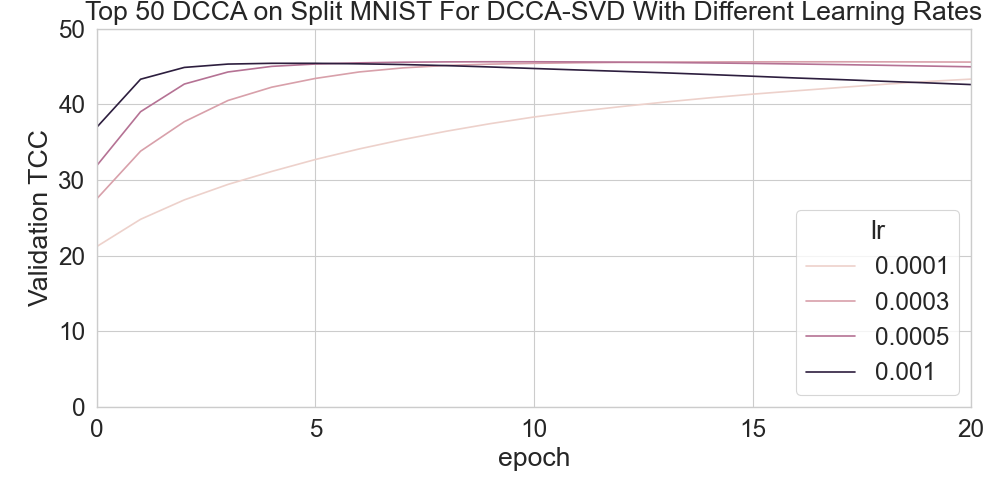
\includegraphics[width=\textwidth]{figures/DCCA/dcca_lr_experiment.png}
         \caption{}
         \label{fig:lrexp}
     \end{subfigure}
     \hfill
     \begin{subfigure}[b]{0.49\textwidth}
         \centering
         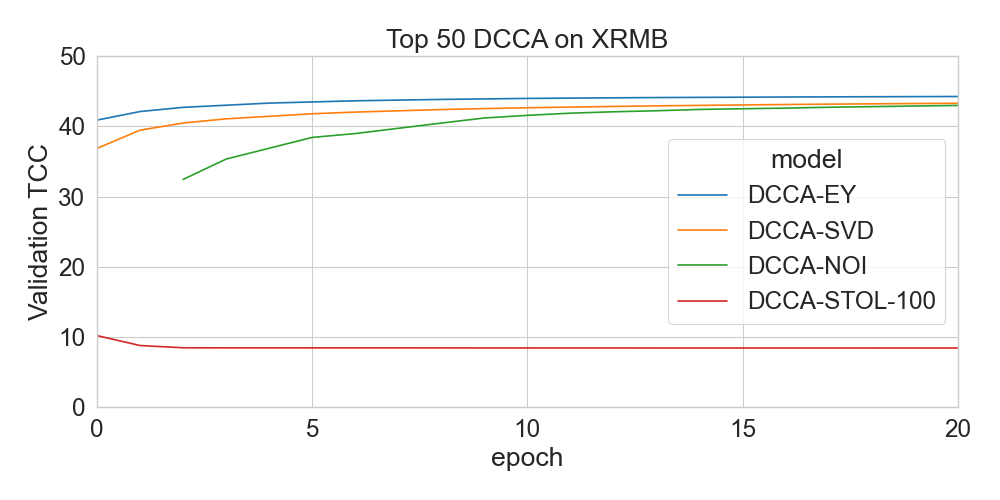
\includegraphics[width=\textwidth]{figures/DCCA/dcca_XRMB.png}
         \caption{}
                 \label{fig:xrmb}
     \end{subfigure}
        \caption{ (a) Validation TCC for different learning rates on Split MNIST data (b) Validation TCC for different methods on XRMB data}

\end{figure}

On the split MNIST data, we show in figure \ref{fig:lrexp} the substantial effect of changing the learning rate on the convergence of the TCC objective. This demonstrates the important of spending computational resource on optimizing the learning rate. An important benefit of our approach is that because the only hyperparameter is learning rate, we can spend all of our computational budget on this critical area. In figure \ref{fig:xrmb}, we show that our proposed methods exhibit extremely fast convergence compared to prior work. Furthermore, both proposed methods find higher validation correlations than DCCA-STOL, showing that they are much more effective ways of estimating the full batch DCCA objective. Note that, the decrease in validation correlation in later epochs is due to overfitting which should be addressed in practical settings by using early stopping as is standard in deep learning.

%%%%%%%%%%%%%%%%%%%%%%%%%%%%%%%%%%%%%%%%%%%%%%%%%%%%%%%%%%%%%%%%%%%%%%%%%%%%%%%%%%%%%%
%SSL
%%%%%%%%%%%%%%%%%%%%%%%%%%%%%%%%%%%%%%%%%%%%%%%%%%%%%%%%%%%%%%%%%%%%%%%%%%%%%%%%%%%%%%
\subsection{Application of SSL-EY and SSL-SVD to Self-Supervised Learning}

In this section, we test our SSL objectives on the CIFAR-10 and CIFAR-100 datasets, which both have 60,000 images and 10 and 100 classes respectively. We compare our methods, SSL-EY and SSL-SVD, with two state-of-the-art methods, Barlow Twins and VICReg. We report k-Nearest Neighbor accuracy on the representations of the validation data in a zero-shot setup.

Firstly, we consider a standard experiment from the literature.
We use the sololearn package \cite{da2022solo}, which includes optimised hyperparameters (and augmentations) for VICReg and Barlow Twins on this specific task.
Each method uses a ResNet-18 encoder, a two-layer projector network with 2048 units in each layer, and is trained for 1,000 epochs with a minibatch size of 256.
For SSL-EY and SSL-SVD, we use the same hyperparameters as Barlow Twins.  
Table \ref{tab:selfsup} shows that our methods are competitive with Barlow Twins and VICReg in this setup.
This is remarkable because their tuning parameters had been heavily optimised, and our method required no tuning at all!

We then performed ablation studies to understand the importance of the (many) hyperparameters in these joint embedding models. In general we found that VICReg was much more sensitive to these hyperparameters than Barlow Twins but that our method was significantly more stable than either of them, see supplement \ref{supp:ablation}.
Table \ref{tab:selfsupsmaller} shows a particularly striking example of this. 
We repeat the previous experiment with all hyperparameters the same apart from the projector: we take a smaller projector with only 256 units in each layer. 
Comparing Tables \ref{tab:selfsup} and \ref{tab:selfsupsmaller} shows that VICReg and Barlow Twins have a large performance drop with the smaller projector on the non-trivial classification problems; our methods are much less affected, and now significantly outperform VICReg and Barlow Twins.


% In this section, we test our SSL objectives empirically on the CIFAR-10 and CIFAR-100 datasets, which both have 60,000 images and 10 and 100 classes respectively. We compare our methods, SSL-EY and SSL-SVD, with two state-of-the-art methods, Barlow Twins and VICReg.

% We use the sololearn package \cite{da2022solo} to reproduce the results of Barlow Twins and VICReg with the optimal augmentations and parameters provided for each method. For SSL-EY and SSL-SVD, we use the same parameters and augmentations as Barlow Twins. Each method uses a minibatch of 256, a ResNet-18 backbone, and a projector network with two layers with 2048 hidden and output units. We train each method for 1,000 epochs and report k-Nearest Neighbor accuracy on the representations of the validation data.

% Table \ref{tab:selfsup} shows that our methods are competitive with Barlow Twins and VICReg in this setup. However, our methods really shine when we reduce the size of the projector network in table \ref{tab:selfsupsmaller}. Since our proposed objectives are based on DCCA, both theory and our earlier ablation studies for DCCA suggest that there is little benefit (in a TCC sense) to using projector outputs with greater dimensionality than the minibatch size (256). To verify this, we repeat the experiment with the same parameters but using a smaller projector with layers and outputs of 256 units. Table \ref{tab:selfsupsmaller} shows the results of this experiment. As expected, and unlike both Barlow Twins and VICReg, we observe only a small difference in performance between experiments with the larger and smaller projectors. 

\begin{table}[h] 
\centering 
\begin{tabular}{lcccc} 
\hline 
Method & CIFAR-10 Top-1 & CIFAR-10 Top-5 & CIFAR-100 Top-1 & CIFAR-100 Top-5 \\ 
\hline 
Barlow Twins & \textbf{92.1} & 99.73 & \textbf{71.38} & \textbf{92.32}\\
VICReg & 91.68	&99.66 & 68.56&	90.76 \\
\textbf{SSL-EY} & 91.43& \textbf{99.75}& 67.52& 90.17\\
\textbf{SSL-SVD} & 90.57 & 99.71 & 65.93 & 89.31 \\
\hline 
\end{tabular} \caption{SSL methods on CIFAR-10 and CIFAR-100 using 2048 unit projectors.} \label{tab:selfsup}
\centering 
\begin{tabular}{lcccc} 
\hline 
Method & CIFAR-10 Top-1 & CIFAR-10 Top-5 & CIFAR-100 Top-1 & CIFAR-100 Top-5 \\ 
\hline 
Barlow Twins & 88.35 & \textbf{99.71} & 59.94 & 85.99 \\
VICReg & 88.74 & 99.68 & 57.03& 84.45 \\
\textbf{SSL-EY} & 89.49 & 99.54 & \textbf{65.62}& \textbf{89.00}\\
\textbf{SSL-SVD} & \textbf{90.34} & 99.67 & 64.54 & 88.66 \\
\hline 
\end{tabular} \caption{SSL methods on CIFAR-10 and CIFAR-100 using 256 unit projectors.} \label{tab:selfsupsmaller} \end{table}

\section{Discussion and Conclusion}





